\chapter{Electronics: Feedback, Oscillators and Signal Acquisition}\label{ch:b2:feedback-oscillators}

Bring a microphone too close to the loudspeaker it feeds and the hall
fills with a howl: the amplifier hears itself, and a tiny noise grows
into a scream at one particular pitch. Tamed, that same loop is the
heart of every clock, radio and synthesizer --- an \emph{oscillator}
that makes a sine wave out of nothing but gain and a filter. The Year 1
volume built amplifiers, filters and comparators with the operational
amplifier; this chapter closes the loop around them, asks when a
loop is stable and when it oscillates, builds two oscillators --- one
sinusoidal, one square --- and then turns to the two operations by
which a measured signal reaches a computer: \emph{sampling} it, and
pulling it out of the noise by \emph{\omterm{prop:b2:feedback-oscillators:lockin}{synchronous detection}}.

\begin{omfigure}
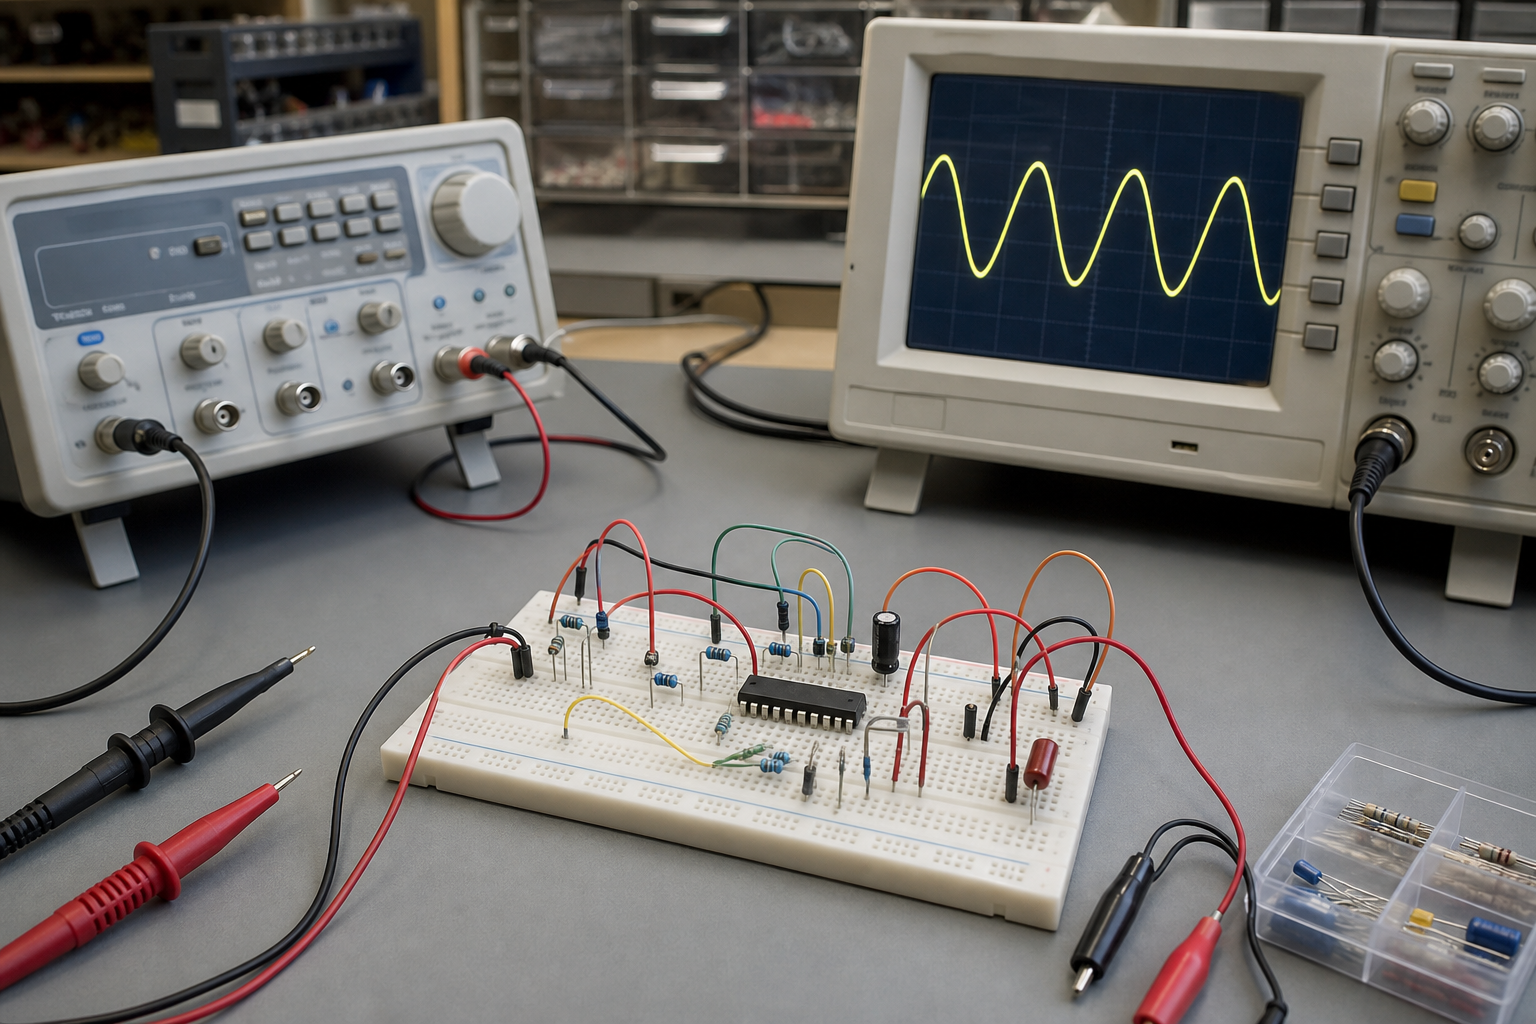
\includegraphics[width=0.58\linewidth]{images/book4/ai/b4-09-electronics-bench-oscillator.png}

{\small A breadboard, a function generator and an oscilloscope: the bench on which a \omterm{def:b2:feedback-oscillators:loop}{feedback} loop is closed --- and on which one discovers, when the amplifier starts to sing, that it has become an oscillator.}
\end{omfigure}


\section{Feedback and stability}

\begin{definition}[Closed loop; loop gain]\label{def:b2:feedback-oscillators:loop}
\index{feedback}\index{loop gain}\index{closed-loop transfer function}
An amplifier of transfer function $\underline A(\jmath\omega)$ receives the
input $\underline e$ plus a fraction $\underline\beta(\jmath\omega)\,\underline s$ of its own
output $\underline s$ (positive feedback; for negative feedback change the
sign of $\beta$). The \emph{closed-loop} transfer function and the
\emph{loop gain} are
\[
\underline H = \frac{\underline s}{\underline e} = \frac{\underline A}{1 - \underline A\,\underline\beta} ,
\qquad \underline T = \underline A\,\underline\beta .
\]
\end{definition}

\begin{theorem}[Stability of a linear loop; oscillation condition]\label{thm:b2:feedback-oscillators:stability}
\index{stability (linear system)}\index{Barkhausen condition}\index{characteristic equation}
Replacing $\jmath\omega$ by the complex variable $p$, the free evolution of
the loop is governed by the roots of its \emph{\omterm{thm:b2:feedback-oscillators:stability}{characteristic equation}}
$1 - \underline A(p)\underline\beta(p) = 0$ (the poles of $\underline H$): each root
$p_i$ contributes a mode $\eu^{p_it}$. The loop is \emph{stable} when all
roots have negative real parts (every mode dies out); it
\emph{oscillates}, with growing amplitude, when a root has a positive
real part. The frontier --- a pair of purely imaginary roots $\pm\jmath
\omega_0$, i.e.\ a sustained sinusoid --- is reached when
\[
\underline A(\jmath\omega_0)\,\underline\beta(\jmath\omega_0) = 1
\]
(\emph{Barkhausen's condition}: \omterm{def:b2:feedback-oscillators:loop}{loop gain} of modulus one and phase
zero at $\omega_0$). For a second-order denominator $ap^2 + bp + c$ the
loop is stable iff $a$, $b$, $c$ have the same sign.
\end{theorem}

\begin{proof}
The differential equation of the loop is obtained from $\underline s(1 -
\underline A\underline\beta) = \underline A\underline e$ by reading each power of $\jmath\omega$
as a time derivative; its homogeneous solutions are the $\eu^{p_it}$
with $p_i$ the roots of the polynomial. Growth or decay follows the
sign of $\operatorname{Re}p_i$; for a second-order polynomial the roots
have negative real parts exactly when the coefficients share one sign
(their sum is $-b/a$ and their product $c/a$). Barkhausen's condition
is the existence of a root at $p = \jmath\omega_0$.
\end{proof}

\begin{remark}[How an oscillator starts and stops]\label{rem:b2:feedback-oscillators:start}
An oscillator is designed with a \omterm{def:b2:feedback-oscillators:loop}{loop gain} slightly \emph{larger} than
one at $\omega_0$: the noise present at switch-on contains that frequency,
which grows exponentially while all others die. Linear theory then
predicts infinite amplitude; in reality some \emph{non-linearity} ---
the saturation of the amplifier, or a deliberately non-linear
element --- lowers the effective gain as the amplitude grows, until the
\omterm{def:b2:feedback-oscillators:loop}{loop gain} averages exactly one: the amplitude settles. Every real
oscillator is thus a linear loop for the frequency and a non-linear
one for the amplitude; the gentler the limiting, the purer the
sine wave.
\end{remark}

\section{The Wien-bridge oscillator}

\begin{proposition}[Wien-bridge oscillator]\label{prop:b2:feedback-oscillators:wien}
\index{Wien-bridge oscillator}\index{Wien network}
An op-amp in the non-inverting configuration of gain $K = 1 + R_2/R_1$
feeds its output back to its $+$ input through the \emph{\omterm{prop:b2:feedback-oscillators:wien}{Wien network}}:
$R$ and $C$ in series, then $R$ and $C$ in parallel to ground. The
network's transfer function is
\[
\underline\beta(\jmath\omega) = \frac1{3 + \jmath(RC\omega - 1/RC\omega)} ,
\]
real and maximal ($= 1/3$) at $\omega_0 = 1/RC$. The \omterm{def:b2:feedback-oscillators:loop}{loop gain} $K\underline\beta$
equals one at $\omega_0$ when $K = 3$: the circuit then sustains a
sinusoid at
\[
f_0 = \frac1{2\pi RC} .
\]
The voltage $v$ at the $+$ input obeys
\[
\frac{\dd^2v}{\dd t^2} + \frac{3 - K}{RC}\,\frac{\dd v}{\dd t} + \frac{v}{R^2C^2} = 0 :
\]
for $K < 3$ the oscillation dies, for $K > 3$ it grows (negative
damping) with the time constant $2RC/(K - 3)$, until the op-amp's
saturation limits it.
\end{proposition}

\begin{proof}
Voltage divider: the series branch $Z_s = R + 1/\jmath C\omega$, the parallel
branch $Z_p = R/(1 + \jmath RC\omega)$; $\underline\beta = Z_p/(Z_s + Z_p)$, which
simplifies to the form given. Loop: $\underline v = \underline\beta K\underline v$, i.e.\
$[3 + \jmath(RC\omega - 1/RC\omega)]\underline v = K\underline v$; multiply by $\jmath\omega RC$
and read $\jmath\omega \to \dd/\dd t$: $R^2C^2\ddot v + (3 - K)RC\dot v + v = 0$.
Its damping coefficient changes sign at $K = 3$.
\end{proof}

\begin{omfigure}
\begin{tikzpicture}[font=\small, x=1cm, y=1cm, >=Stealth, scale=0.9, every node/.style={transform shape}]
  \begin{scope}
    \node[draw, thick, minimum width=1.4cm, minimum height=0.8cm] (A) at (0,0) {$\underline A$};
    \node[draw, thick, minimum width=1.4cm, minimum height=0.8cm] (B) at (0,-1.7) {$\underline\beta$};
    \draw[thick] (-2.3,0) circle (0.2); \node at (-2.3,0) {$+$};
    \draw[thick, ->] (-3.2,0) -- (-2.5,0) node[above, pos=0.3, font=\footnotesize] {$\underline e$};
    \draw[thick, ->] (-2.1,0) -- (A.west);
    \draw[thick, ->] (A.east) -- (2.0,0) node[above, pos=0.6, font=\footnotesize] {$\underline s$};
    \draw[thick] (1.4,0) -- (1.4,-1.7) -- (B.east);
    \draw[thick, ->] (B.west) -- (-2.3,-1.7) -- (-2.3,-0.2);
    \node[font=\footnotesize] at (-0.3,-2.7) {$\underline H = \dfrac{\underline A}{1 - \underline A\underline\beta}$};
  \end{scope}
\end{tikzpicture}
\hfill
\begin{tikzpicture}[font=\small, scale=0.78, every node/.style={transform shape}]
    \draw (0,0) node[op amp, noinv input down] (oa) {};
    % negative feedback: R2 from output to - input, R1 from - input to ground
    \coordinate (M) at ($(oa.-)+(-0.7,0)$);
    \draw (oa.-) -- (M);
    \draw (M) to[R, l_=$R_1$] ++(-1.6,0) node[ground, rotate=-90]{};
    \draw (M) -- ++(0,1.4) coordinate (T) to[R, l=$R_2$] (T -| oa.out) -- (oa.out);
    % Wien network: from output down, series C and R to node P, P to + input; P to ground via R and via C
    \coordinate (P) at (-3.4,-2.3);
    \draw (oa.out) -- ++(0.6,0) coordinate (O) -- (O |- P) to[C, l=$C$] ++(-1.6,0) to[R, l=$R$] (P);
    \draw (P) -- (P |- oa.+) -- (oa.+);
    \draw (P) to[R, l_=$R$] ++(0,-1.6) node[ground]{};
    \draw (P) -- ++(-1.1,0) coordinate (Q) to[C, l_=$C$] ++(0,-1.6) node[ground]{};
    \draw (O) to[short, -o] ++(0.5,0) node[right, font=\footnotesize] {$s$};
\end{tikzpicture}

{\small Left: a \omterm{def:b2:feedback-oscillators:loop}{feedback} loop --- the output is fed back, through
$\underline\beta$, to the input of the amplifier. Right: the \omterm{prop:b2:feedback-oscillators:wien}{Wien-bridge
oscillator} --- a non-inverting amplifier of gain $1 + R_2/R_1$ whose
output returns to its $+$ input through the series--parallel $RC$
network; it oscillates at $1/2\pi RC$ when the gain reaches 3.}
\end{omfigure}

\begin{example}[A 1 kHz source]\label{ex:b2:feedback-oscillators:wiennumbers}
$R = \qty{15.9}{k\ohm}$, $C = \qty{10}{nF}$: $f_0 = \qty{1.00}{kHz}$. With $R_1 =
\qty{10}{k\ohm}$ and $R_2 = \qty{21}{k\ohm}$, $K = 3.1$: the amplitude grows by
$\eu$ every $2RC/0.1 = \qty{3.2}{ms}$ from the switch-on noise, reaching
saturation in a few tens of milliseconds; the clipped sine is then
rich in harmonics. Replacing $R_1$ by a small incandescent lamp, whose
resistance rises as it warms, pulls $K$ down to exactly $3$ at a
moderate amplitude: a sine wave with less than $0.1\%$ of distortion,
the circuit of the first laboratory signal generators.
\end{example}

\section{Comparators with hysteresis; the astable multivibrator}

\begin{proposition}[Hysteresis comparator]\label{prop:b2:feedback-oscillators:schmitt}
\index{hysteresis comparator}\index{Schmitt trigger}
An op-amp with \emph{positive} \omterm{def:b2:feedback-oscillators:loop}{feedback} --- output fed to the $+$ input
through a divider $R_1$, $R_2$ (the $+$ input then sits at $\beta s$ with
$\beta = R_1/(R_1 + R_2)$ when the signal $e$ is applied to the $-$ input)
--- has no stable linear regime: its output sits at $+V_{\text{sat}}$ or
$-V_{\text{sat}}$ and switches
\begin{align*}
&\text{from } +V_{\text{sat}} \text{ to } -V_{\text{sat}} \text{ when } e \text{ rises above } +\beta V_{\text{sat}} ,\\
&\text{from } -V_{\text{sat}} \text{ to } +V_{\text{sat}} \text{ when } e \text{ falls below } -\beta V_{\text{sat}} .
\end{align*}
The two thresholds differ: the \emph{hysteresis} $2\beta V_{\text{sat}}$ makes
the comparator immune to noise smaller than that, and its cycle in
the $(e, s)$ plane is a rectangle run clockwise.
\end{proposition}

\begin{proof}
With $s = +V_{\text{sat}}$ the $+$ input is at $+\beta V_{\text{sat}}$; the output
stays positive as long as $e < \beta V_{\text{sat}}$, and flips when $e$ crosses
it --- after which the $+$ input is at $-\beta V_{\text{sat}}$, so $e$ must
fall below that to flip it back. (In the linear regime the positive
\omterm{def:b2:feedback-oscillators:loop}{feedback} would make any deviation grow: it is unstable.)
\end{proof}

\begin{proposition}[Astable multivibrator]\label{prop:b2:feedback-oscillators:astable}
\index{astable multivibrator}\index{relaxation oscillator}
Feed the output of the \omterm{prop:b2:feedback-oscillators:schmitt}{hysteresis comparator} back to its own $-$ input
through an $RC$ circuit ($R$ from $s$ to the $-$ input, $C$ from there
to ground). The capacitor charges toward $\pm V_{\text{sat}}$ and flips the
comparator each time it reaches a threshold: a square wave at $s$, a
near-triangular wave on $C$, with the period
\[
T = 2RC\,\ln\frac{1 + \beta}{1 - \beta} .
\]
For $\beta = 1/2$, $T = 2RC\ln3 \approx 2.2RC$. Such \emph{\omterm{prop:b2:feedback-oscillators:astable}{relaxation
oscillators}} clock microcontrollers, blink indicators and generate
the triangle and square waves of function generators.
\end{proposition}

\begin{proof}
With $s = +V_{\text{sat}}$, the capacitor voltage $v_C$ goes from
$-\beta V_{\text{sat}}$ toward $+V_{\text{sat}}$ as $v_C = V_{\text{sat}} - (1 + \beta)
V_{\text{sat}}\eu^{-t/RC}$, and reaches $+\beta V_{\text{sat}}$ after $RC\ln[(1 + \beta)
/(1 - \beta)]$; the comparator flips and the symmetric half-cycle follows.
\end{proof}

\begin{omfigure}
\begin{tikzpicture}
\begin{axis}[omaxis, axis x line=middle, axis y line=middle, width=5.6cm, height=4.6cm,
    xlabel={$e$}, ylabel={$s$}, xmin=-1.6, xmax=1.6, ymin=-1.5, ymax=1.5,
    xtick=\empty, ytick=\empty, clip=false]
  \node[font=\scriptsize, anchor=north] at (axis cs:-0.5,-1.55) {$-\beta V_{\text{sat}}$};
  \node[font=\scriptsize, anchor=north] at (axis cs:0.5,-1.55) {$\beta V_{\text{sat}}$};
  \node[font=\scriptsize, anchor=east] at (axis cs:-1.55,1) {$V_{\text{sat}}$};
  \node[font=\scriptsize, anchor=east] at (axis cs:-1.55,-1) {$-V_{\text{sat}}$};
  \draw[dotted] (axis cs:-0.5,0) -- (axis cs:-0.5,-1.5); \draw[dotted] (axis cs:0.5,0) -- (axis cs:0.5,-1.5);
  \addplot[omDef, very thick] coordinates {(-1.5,1) (0.5,1)};
  \addplot[omDef, very thick, ->] coordinates {(0.5,1) (0.5,-1)};
  \addplot[omDef, very thick] coordinates {(0.5,-1) (-0.5,-1)};
  \addplot[omDef, very thick, ->] coordinates {(-0.5,-1) (-0.5,1)};
  \addplot[omDef, very thick] coordinates {(-0.5,-1) (1.5,-1)};
\end{axis}
\end{tikzpicture}
\hfill
\begin{tikzpicture}
\begin{axis}[omaxis, axis x line=middle, axis y line=left, width=8.0cm, height=4.6cm,
    xlabel={$t$}, ylabel={}, xmin=0, xmax=4.4, ymin=-1.4, ymax=1.4, xtick=\empty, ytick={-1,-0.5,0.5,1},
    yticklabels={$-V_{\text{sat}}$, $-\beta V_{\text{sat}}$, $\beta V_{\text{sat}}$, $V_{\text{sat}}$}, tick label style={font=\scriptsize}, samples=60,
    xlabel style={at={(axis description cs:1.0,0.5)}, anchor=west},
    legend style={font=\scriptsize, at={(0.5,1.02)}, anchor=south, legend columns=2, draw=none, fill=none}]
  \addplot[omThm, thick] coordinates {(0,1) (1.1,1) (1.1,-1) (2.2,-1) (2.2,1) (3.3,1) (3.3,-1) (4.4,-1)};
  \addplot[omDef, thick, domain=0:1.1] {1-1.5*exp(-x)};
  \addplot[omDef, thick, domain=1.1:2.2] {-1+1.5*exp(-(x-1.1))};
  \addplot[omDef, thick, domain=2.2:3.3] {1-1.5*exp(-(x-2.2))};
  \addplot[omDef, thick, domain=3.3:4.4] {-1+1.5*exp(-(x-3.3))};
  \legend{$s$ (square), $v_C$}
\end{axis}
\end{tikzpicture}

{\small Left: the cycle of a \omterm{prop:b2:feedback-oscillators:schmitt}{hysteresis comparator} --- two thresholds,
a rectangle run clockwise. Right: the \omterm{prop:b2:feedback-oscillators:astable}{astable multivibrator} ---
the capacitor voltage shuttles between the thresholds and the output is
a square wave.}
\end{omfigure}

\section{Sampling a signal}

\begin{theorem}[Sampling; the Nyquist--Shannon criterion]\label{thm:b2:feedback-oscillators:shannon}
\index{sampling}\index{Nyquist--Shannon criterion}\index{aliasing}\index{anti-aliasing filter}
A signal is \emph{sampled} when only its values $s(nT_s)$ at the
instants $nT_s$ are kept, $f_s = 1/T_s$ being the \emph{sampling rate}.
The spectrum of the sampled signal is the spectrum of $s$ repeated
around every multiple of $f_s$. A signal whose spectrum is confined
below $f_{\max}$ can be exactly reconstructed from its samples if and
only if
\[
f_s > 2f_{\max} ;
\]
otherwise the copies overlap and a component at $f > f_s/2$ reappears
at the \emph{alias} frequency $|f - nf_s|$ (for the integer $n$ that
brings it below $f_s/2$), indistinguishable from a true low-frequency
component. Hence the \emph{\omterm{thm:b2:feedback-oscillators:shannon}{anti-aliasing filter}} placed before any
sampler: a low-pass that removes everything above $f_s/2$.
\end{theorem}

\begin{proof}
Sampling is multiplying $s(t)$ by a periodic train of narrow pulses of
period $T_s$, whose Fourier series contains all the harmonics $nf_s$
(the mathematics volume of this year); multiplying $s$ by $\cos(2\pi nf_st)$
shifts its spectrum by $\pm nf_s$ --- whence the copies. They do not
overlap iff $f_{\max} < f_s - f_{\max}$; a low-pass of cut-off $f_s/2$ then
recovers the original spectrum exactly (admitted). Aliasing: the
samples of $\cos(2\pi ft)$ and of $\cos(2\pi(f - nf_s)t)$ at $t = mT_s$
coincide, since $2\pi nf_smT_s = 2\pi nm$.
\end{proof}

\begin{example}[Wagon wheels, CDs and oscilloscopes]\label{ex:b2:feedback-oscillators:alias}
A film at $24$ images per second samples the world at \qty{24}{Hz}: a
wheel with $12$ spokes turning at $2.1$ turns per second presents a spoke
$25.2$ times a second, $1.2$ beyond $f_s$ --- it seems to turn slowly
forward, and backward at $1.9$ turns per second. A compact disc samples
at \qty{44.1}{kHz} to reproduce sound up to \qty{20}{kHz}, with a steep
\omterm{thm:b2:feedback-oscillators:shannon}{anti-aliasing filter} between $20$ and \qty{22}{kHz}. A digital oscilloscope
set to \qty{1}{MS/s} displays a \qty{999}{kHz} sine as a \qty{1}{kHz} one ---
the first trap of digital measurement.
\end{example}

\begin{omfigure}
\begin{tikzpicture}
\begin{axis}[omaxis, axis x line=middle, axis y line=none, width=13.6cm, height=4.0cm,
    xmin=0, xmax=10, ymin=-1.4, ymax=1.5, xtick=\empty, samples=400, xlabel={$t$},
    xlabel style={at={(axis description cs:1.0,0.5)}, anchor=west},
    legend style={font=\scriptsize, at={(0.5,1.02)}, anchor=south, legend columns=3, draw=none, fill=none}]
  \addplot[omDef, thick, domain=0:10] {cos(deg(2*pi*0.9*x))};
  \addplot[omThm, thick, dashed, domain=0:10] {cos(deg(2*pi*0.1*x))};
  \addplot[only marks, mark=*, mark size=1.6pt, black, samples=11, domain=0:10] {cos(deg(2*pi*0.9*x))};
  \legend{$f = 0.9f_s$, alias at $0.1f_s$, samples}
\end{axis}
\end{tikzpicture}

{\small Aliasing: a sinusoid at $0.9f_s$ and one at $0.1f_s$ pass through
the same samples; once sampled, they cannot be told apart --- hence the
criterion $f_s > 2f_{\max}$.}
\end{omfigure}

\begin{remark}[Quantization]\label{rem:b2:feedback-oscillators:quantization}
\index{quantization}\index{analog-to-digital converter}
The \omterm{rem:b2:feedback-oscillators:quantization}{analog-to-digital converter} also rounds each sample to one of
$2^N$ levels ($N$ bits): the rounding error, at most half a step, acts
as a noise of rms value $\Delta/\sqrt{12}$ for a step $\Delta$, and the
dynamic range (largest sine over that noise) is about $6N + 2$ dB ---
\qty{98}{dB} for the $16$ bits of a CD, \qty{74}{dB} for a $12$-bit
oscilloscope. Sampling rate and resolution are the two numbers on the
label of every digitizer.
\end{remark}

\section{Synchronous detection}

\begin{proposition}[Synchronous (lock-in) detection]\label{prop:b2:feedback-oscillators:lockin}
\index{synchronous detection}\index{lock-in amplifier}\index{demodulation}
A signal of known frequency, $s(t) = A\cos(\omega_0t + \varphi)$, buried in a
noise $n(t)$ of much larger amplitude spread over a wide band, is
multiplied by a reference $r(t) = \cos\omega_0t$ of the same frequency
and passed through a low-pass filter of cut-off $f_c \ll f_0$:
\[
s(t)r(t) = \tfrac12A\cos\varphi + \tfrac12A\cos(2\omega_0t + \varphi)
\ \xrightarrow{\ \text{low-pass}\ }\ \tfrac12A\cos\varphi .
\]
The output is a DC voltage proportional to the signal's amplitude (and
to the cosine of its phase relative to the reference), while the noise
is reduced to the part of its spectrum lying within $\pm f_c$ of $f_0$
--- a bandwidth $2f_c$ that can be made arbitrarily narrow (a fraction
of a hertz for a filter time constant of seconds). Components at other
frequencies $f$ are shifted to $f \pm f_0$ and rejected by the filter.
\end{proposition}

\begin{proof}
$\cos a\cos b = \tfrac12[\cos(a - b) + \cos(a + b)]$; the filter keeps the
difference term for the signal, the $2\omega_0$ term and every noise
component at $f$ being shifted to $|f - f_0|$ and $f + f_0$ --- only the
noise originally within $f_c$ of $f_0$ lands below $f_c$.
\end{proof}

\begin{omfigure}
\begin{tikzpicture}[font=\small, x=1cm, y=1cm, >=Stealth]
  \node[draw, thick, minimum width=1.5cm, minimum height=0.8cm] (S) at (0,0) {sensor};
  \node[draw, thick, circle, minimum size=0.7cm] (M) at (2.6,0) {$\times$};
  \node[draw, thick, minimum width=1.6cm, minimum height=0.8cm] (F) at (5.0,0) {low-pass};
  \node[draw, thick, minimum width=1.7cm, minimum height=0.8cm] (R) at (2.6,-1.9) {reference $\omega_0$};
  \draw[thick, ->] (S) -- (M) node[above, pos=0.5, font=\footnotesize] {$s + n$};
  \draw[thick, ->] (M) -- (F);
  \draw[thick, ->] (F) -- (7.0,0) node[right, font=\footnotesize] {$\tfrac12A\cos\varphi$};
  \draw[thick, ->] (R) -- (M);
  \draw[thick, ->] (R.west) -- (-0.2,-1.9) -- (-0.2,-0.5) node[left, font=\footnotesize, pos=0.5] {modulates};
\end{tikzpicture}
\hfill
\begin{tikzpicture}
\begin{axis}[omaxis, axis x line=bottom, axis y line=left, width=5.6cm, height=4.0cm,
    xlabel={$f$}, ylabel={}, xmin=0, xmax=3, ymin=0, ymax=1.3, xtick={1,2}, xticklabels={$f_0$, $2f_0$}, ytick=\empty, samples=200,
    xlabel style={at={(axis description cs:1.0,0.0)}, anchor=west}]
  \addplot[omExo!60, thick, domain=0:3] {0.35+0.1*sin(deg(11*x))+0.08*cos(deg(23*x))};
  \addplot[omThm, very thick] coordinates {(1,0) (1,1.1)};
  \addplot[omDef, thick, fill=omDef!30, domain=0.9:1.1] {1.2} \closedcycle;
  \node[font=\scriptsize, omDef, anchor=west] at (axis cs:1.15,1.15) {kept};
  \node[font=\scriptsize] at (axis cs:2.2,0.6) {noise};
\end{axis}
\end{tikzpicture}

{\small \omterm{prop:b2:feedback-oscillators:lockin}{Synchronous detection}: the sensor's output, signal plus broad
noise, is multiplied by a reference at the signal's own frequency and
low-pass filtered; only the noise within a narrow band around $f_0$
(shaded) survives, and the signal comes out as a DC level.}
\end{omfigure}

\begin{example}[Finding a microvolt]\label{ex:b2:feedback-oscillators:microvolt}
A photodiode delivers \qty{10}{\micro V} of signal when its light is chopped
at \qty{1}{kHz}, on top of \qty{50}{nV/\sqrt{Hz}} of white noise over
\qty{100}{kHz} (\qty{16}{\micro V} rms: more than the signal). After \omterm{prop:b2:feedback-oscillators:lockin}{synchronous
detection} with a filter of time constant $\tau = \qty{1}{s}$ (noise
bandwidth $1/4\tau = \qty{0.25}{Hz}$) the noise is $50\,\text{nV} \times \sqrt{0.25}
= \qty{25}{nV}$: a signal-to-noise ratio of $400$ --- at the price of
waiting a few seconds per point. The same trick, under the name of
\emph{demodulation}, recovers the music from an AM radio carrier and
the data from a modem.
\end{example}

\begin{method}[Designing a measurement chain]\label{met:b2:feedback-oscillators:method}
(1) Modulate the quantity to be measured at a frequency $f_0$ away from
the noise (chopper, AC bridge). (2) Amplify with a bandwidth covering
$f_0$. (3) Detect synchronously with a filter whose time constant is
the longest the measurement can afford: the noise falls as
$1/\sqrt\tau$. (4) Sample the slow output at a rate above twice its
bandwidth, after an \omterm{thm:b2:feedback-oscillators:shannon}{anti-aliasing filter}, with enough bits for the
required resolution. (5) Check the chain with a known signal, and that
nothing in it oscillates: every amplifier with \omterm{def:b2:feedback-oscillators:loop}{feedback} is a potential
oscillator.
\end{method}

\section{Exercises}

\begin{exercise}[$\star$]\label{exo:b2:feedback-oscillators:1}
A \omterm{prop:b2:feedback-oscillators:wien}{Wien-bridge oscillator} with $R = \qty{10}{k\ohm}$, $C = \qty{10}{nF}$:
frequency; gain needed; values of $R_1$, $R_2$ for $K = 3.05$ with $R_1 =
\qty{10}{k\ohm}$; time constant of the amplitude growth. Which components
fix the frequency, which the start-up?
\end{exercise}

\begin{exercise}[$\star$]\label{exo:b2:feedback-oscillators:2}
\omterm{prop:b2:feedback-oscillators:schmitt}{Hysteresis comparator} with $V_{\text{sat}} = \qty{\pm 13}{V}$, $R_1 = \qty{1.0}{k\ohm}$,
$R_2 = \qty{4.0}{k\ohm}$: thresholds, hysteresis width. A noisy signal
crossing zero with \qty{2}{V} of noise: how many times does the output
switch per crossing, with and without hysteresis?
\end{exercise}

\begin{exercise}[$\star$]\label{exo:b2:feedback-oscillators:3}
\omterm{prop:b2:feedback-oscillators:astable}{Astable multivibrator} with $R = \qty{10}{k\ohm}$, $C = \qty{100}{nF}$, $\beta = 0.5$:
period and frequency; $R$ for \qty{1.0}{kHz}; amplitude of the triangular
wave on the capacitor; what happens to $T$ if $\beta$ is raised to $0.9$?
\end{exercise}

\begin{exercise}[$\star$]\label{exo:b2:feedback-oscillators:4}
(a) A CD samples at \qty{44.1}{kHz}: maximum frequency reproduced. (b) A
\qty{30}{kHz} ultrasound leaks into the recording: at what frequency does
it appear? (c) A wheel with $8$ spokes filmed at \qty{25}{images/s} turns
at $3.2$ turns/s: apparent motion. (d) An oscilloscope at \qty{10}{MS/s}
shows a clean \qty{100}{kHz} sine; the true signal could be what other
frequencies?
\end{exercise}

\begin{exercise}[$\star\star$]\label{exo:b2:feedback-oscillators:5}
Loops with characteristic polynomials (a) $p^2 + 3p + 2$, (b) $p^2 - p +
4$, (c) $p^2 + 4$, (d) $p^3 + 2p^2 + 2p + 1$, (e) $p^3 + p + 1$: find or
discuss the roots; which loops are stable, which oscillate, which grow?
(For the cubics, reason on the sign of the real parts: e.g.\ show (e)
has a real negative root and two complex roots with positive real
part, using the product and sum of the roots.)
\end{exercise}

\begin{exercise}[$\star\star$]\label{exo:b2:feedback-oscillators:6}
\emph{\omterm{prop:b2:feedback-oscillators:wien}{Wien network}.} (a) Derive $\underline\beta(\jmath\omega)$ from the divider.
(b) Plot (sketch) its modulus and phase; show the phase is zero only at
$\omega_0$ and that the modulus is then $1/3$. (c) Write the differential
equation of the loop for a gain $K$ and discuss $K < 3$, $K = 3$, $K > 3$.
(d) With $K = 3.2$, starting from a \qty{1}{mV} noise, how long until the
amplitude reaches \qty{10}{V}? Why does the final amplitude not depend on
the initial noise?
\end{exercise}

\begin{exercise}[$\star\star$]\label{exo:b2:feedback-oscillators:7}
\emph{Triangle generator.} An integrator (op-amp, $R$, $C$) is fed by
the square output $\pm V_{\text{sat}}$ of a \omterm{prop:b2:feedback-oscillators:schmitt}{hysteresis comparator} whose input
is the integrator's output; the comparator thresholds are
$\pm V_{\text{sat}}R_1/R_2$. (a) Show the integrator output is a triangle;
its slope. (b) Period $T = 4RCR_1/R_2$. (c) Numbers: $R = \qty{10}{k\ohm}$,
$C = \qty{10}{nF}$, $R_1/R_2 = 0.5$. (d) Advantage over the simple astable
for a function generator.
\end{exercise}

\begin{exercise}[$\star\star$]\label{exo:b2:feedback-oscillators:8}
Quantization. (a) A $16$-bit converter on $\pm\qty{1}{V}$: step, rms
quantization noise, dynamic range in dB. (b) $12$ bits at
\qty{1}{MS/s}: bit rate; same for $8$ bits at \qty{1}{GS/s} (a fast
oscilloscope). (c) A \qty{1}{mV} signal on the $16$-bit converter: how many
steps? What to do before the converter? (d) Why does a good audio
system dither (add a little noise) before quantizing?
\end{exercise}

\begin{exercise}[$\star\star$]\label{exo:b2:feedback-oscillators:9}
A signal contains \qty{1.0}{kHz} and \qty{9.0}{kHz} components and is
sampled at \qty{10}{kS/s}. (a) Where does each appear? (b) An
anti-aliasing first-order $RC$ filter with $f_c = \qty{2}{kHz}$ is added:
\omterm{def:b2:dispersion-wave-packets:complex}{attenuation} at \qty{9}{kHz} in dB; enough if \qty{40}{dB} is wanted? (c)
Order of the filter needed (\omterm{def:b2:dispersion-wave-packets:complex}{attenuation} $\approx 20n$ dB per decade); or,
alternatively, sampling rate needed with the first-order filter. (d)
Why do modern converters oversample and filter digitally?
\end{exercise}

\begin{exercise}[$\star\star\star$]\label{exo:b2:feedback-oscillators:10}
\emph{Lock-in.} Input $A\cos(\omega_0t + \varphi) + n(t)$ multiplied by $\cos\omega_0t$
and filtered by a first-order low-pass of time constant $\tau$. (a) DC
output. (b) Show that a noise component at $f = f_0 + \delta f$ gives, after
the filter, an amplitude reduced by $1/\sqrt{1 + (2\pi\delta f\tau)^2}$;
deduce the equivalent noise bandwidth $B = 1/4\tau$ (admit $\int_0^\infty
\dd x/(1 + x^2) = \pi/2$). (c) A \qty{1}{\micro V} signal in \qty{1}{mV} rms of
white noise over \qty{10}{kHz}: noise density; $\tau$ for a signal-to-noise
ratio of $10$; measuring time. (d) A \qty{50}{Hz} pickup of \qty{1}{mV}
pollutes the input, with $f_0 = \qty{1}{kHz}$: where does it go, and by
how much is it attenuated for $\tau = \qty{1}{s}$?
\end{exercise}

\begin{exercise}[$\star\star\star$]\label{exo:b2:feedback-oscillators:11}
\emph{Quartz.} A quartz crystal behaves, near its resonance, as a
series $L$, $C$, $r$ branch ($L = \qty{8000}{H}$, $C = \qty{3.0}{fF}$, $r =
\qty{30}{k\ohm}$) in parallel with $C_0 = \qty{1.5}{pF}$. (a) Series resonance
frequency and quality factor $Q = L\omega_0/r$. (b) Why does an oscillator
built around it hold its frequency to a part in $10^6$ while the Wien
bridge drifts by percent (think of the phase slope $\dd\varphi/\dd\omega$ of
the \omterm{def:b2:feedback-oscillators:loop}{feedback} network near resonance, $\sim 2Q/\omega_0$)? (c) A watch
crystal at \qty{32768}{Hz} is divided by $2^{15}$: result; its frequency
varies as $-0.04\,\text{ppm}\,(T - \qty{25}{\degreeCelsius})^2$: error per
month at \qty{5}{\degreeCelsius}. (d) Why is \qty{32768}{Hz} chosen and not
\qty{1}{MHz}?
\end{exercise}

\begin{exercise}[$\star\star\star$]\label{exo:b2:feedback-oscillators:12}
\emph{Negative resistance.} An op-amp has $R_2$ from output to $-$
input, $R_1$ from $-$ input to ground, and $R$ from output to $+$ input;
the dipole seen between the $+$ input and ground is studied (linear
regime). (a) Show that it behaves as a resistance $-RR_1/R_2$. (b) This
dipole is connected across a parallel $LC$ circuit of loss resistance
$R_p$ (in parallel): write the equation of the voltage and find the
condition for sustained oscillation and the frequency. (c) Numbers: $L
= \qty{10}{mH}$, $C = \qty{100}{nF}$, $R_p = \qty{50}{k\ohm}$; choose $R$, $R_1 =
R_2$. (d) What limits the amplitude, and how does this oscillator
compare with the Wien bridge?
\end{exercise}

\section{Problem: A lock-in measurement chain}

\begin{problem}[{Weekend problem --- from the reference oscillator to the
digitized result: measuring ten microvolts of light signal under a
millivolt of noise}]
\label{pb:b2:feedback-oscillators:1}

A faint light is to be measured with a photodiode. The light is chopped
by a rotating wheel at $f_0 = \qty{1.00}{kHz}$, so that the photodiode's
output is a sinusoid of amplitude $A = \qty{10}{\micro V}$ at $f_0$ (after a
first amplifier), on which rides a white noise of spectral density
$e_n = \qty{50}{nV/\sqrt{Hz}}$ over a bandwidth of \qty{100}{kHz}, plus a
\qty{50}{Hz} mains pickup of \qty{1.0}{mV}. The chopper's own frequency is
set by a \omterm{prop:b2:feedback-oscillators:wien}{Wien-bridge oscillator}.

\medskip
\noindent\textbf{Part I --- The reference oscillator.}
Wien bridge with $C = \qty{10}{nF}$, op-amp saturating at $\pm\qty{12}{V}$.
\begin{enumerate}
  \item $R$ for $f_0 = \qty{1.00}{kHz}$.
  \item Derive the transfer function of the \omterm{prop:b2:feedback-oscillators:wien}{Wien network} and check
        that its phase vanishes at $f_0$ with modulus $1/3$.
  \item Write the differential equation of the loop for a gain $K$; for
        $K = 3.15$, time for the amplitude to grow by a factor $1000$.
  \item The amplitude is finally limited by saturation: describe the
        waveform, and why its harmonics matter for a reference.
  \item A thermistor in place of $R_1$ (resistance falling when it
        warms) or a lamp (rising): which one stabilizes the gain at 3,
        and how?
  \item The capacitors drift by $+1\%$ with temperature: new frequency.
        Why does the chopper then still work for the measurement (what
        must the reference do)?
  \item The \omterm{prop:b2:feedback-oscillators:wien}{Wien network} has a quality factor of about $1/3$: what does
        that imply for the purity of the frequency compared with a
        quartz ($Q \sim 10^5$)?
\end{enumerate}

\medskip
\noindent\textbf{Part II --- The signal and the noise.}
\begin{enumerate}[resume]
  \item Rms value of the white noise over the full \qty{100}{kHz};
        signal-to-noise ratio at the amplifier output.
  \item A band-pass filter of quality factor $Q = 10$ centred on $f_0$
        (noise bandwidth $\approx f_0/Q$) is inserted: noise rms and SNR.
        Why is this not sufficient for a precise measurement (think of
        drifts and of the \qty{50}{Hz})?
  \item Why chop the light at \qty{1}{kHz} instead of measuring the DC
        photocurrent directly? (Amplifiers have "$1/f$" noise rising
        below a few hundred hertz.)
  \item Signal amplitude if the chopper wheel produces a square
        modulation instead of a sine: which harmonic does the lock-in
        keep, and with what amplitude (Fourier coefficient $4/\pi$ for the
        fundamental of a square wave of unit amplitude)?
  \item The photodiode also receives room light at \qty{100}{Hz}
        (fluorescent tubes): what does the chain do with it?
\end{enumerate}

\medskip
\noindent\textbf{Part III --- \omterm{prop:b2:feedback-oscillators:lockin}{Synchronous detection}.}
The amplified signal is multiplied by the reference $\cos(2\pi f_0t)$
and filtered by a first-order low-pass of time constant $\tau$.
\begin{enumerate}[resume]
  \item Output of the multiplier for the signal alone (phase $\varphi$
        between signal and reference); the DC term.
  \item \omterm{def:b2:dispersion-wave-packets:complex}{Attenuation} of the $2f_0$ term by the filter for $\tau = \qty{1}{s}$
        (in dB).
  \item Equivalent noise bandwidth $1/4\tau$; rms noise at the output
        for $\tau = \qty{1}{s}$ and the SNR; same for $\tau = \qty{10}{s}$.
  \item Where does the \qty{50}{Hz} pickup end up, and with what
        \omterm{def:b2:dispersion-wave-packets:complex}{attenuation} for $\tau = \qty{1}{s}$?
  \item The phase $\varphi$ is unknown: what is lost if $\varphi = \qty{60}{\degree}$?
        Describe the two-channel (in-phase and quadrature) lock-in and
        how it recovers $A$ whatever $\varphi$.
  \item Response time of the measurement (time to reach $99\%$ of the
        final value) for $\tau = \qty{1}{s}$; the trade-off it expresses.
  \item The reference drifts to \qty{1001}{Hz} while the chopper stays at
        \qty{1000}{Hz}: output of the lock-in; why the reference must be
        taken from the chopper itself.
\end{enumerate}

\medskip
\noindent\textbf{Part IV --- Digitizing.}
\begin{enumerate}[resume]
  \item The lock-in output is sampled by a computer: minimum rate for
        $\tau = \qty{1}{s}$ (take the output bandwidth as $1/2\pi\tau$); a
        comfortable choice.
  \item Alternatively the raw \qty{1}{kHz} signal is digitized and the
        detection done in software: minimum sampling rate; the noise
        extends to \qty{100}{kHz} --- what must be done before sampling,
        and what \omterm{def:b2:dispersion-wave-packets:complex}{attenuation} at \qty{100}{kHz} does a sampling at
        \qty{20}{kS/s} with a fourth-order filter cut at \qty{5}{kHz} give
        (\qty{80}{dB} per decade)?
  \item A $16$-bit converter on $\pm\qty{1}{V}$: step; the \qty{10}{\micro V}
        signal amplified by $1000$: how many steps, and does the noise
        help or hurt?
  \item Digital lock-in: the computer multiplies each sample by
        $\cos(2\pi f_0nT_s)$ and averages $N$ samples. At \qty{20}{kS/s},
        $N$ for a \qty{1}{s} average; by what factor is the white noise
        reduced, and is it the same as the analog filter's?
  \item A \qty{1}{kHz} signal sampled at \qty{999}{S/s}: what does the
        computer see? How does this relate to the lock-in's own
        principle?
  \item Summarize the chain in a table: each stage, what it does to the
        signal, what it does to the noise.
\end{enumerate}
\end{problem}
